\qrchapter{https://forgottenpillar.com/rsc/en-fp-chapter21}{Remembering the beginning} \label{chap:remembering-the-beginning}


\qrchapter{https://forgottenpillar.com/rsc/en-fp-chapter21}{Recordando el principio} \label{chap:remembering-the-beginning}


\egw{\textbf{We cannot for a moment have any \underline{misrepresentation} upon these solemn and important subjects of truth which have been the faith of our people since 1844.}}[Lt300-1903.9; 1903][https://egwwritings.org/read?panels=p7705.15]


\egw{\textbf{No podemos por un momento tener ninguna \underline{tergiversación} sobre estos solemnes e importantes temas de la verdad que han sido la fe de nuestro pueblo desde 1844.}}[Lt300-1903.9; 1903][https://egwwritings.org/read?panels=p7705.15]


The true meaning of the \emcap{Fundamental Principles} is a broader view of the three angels’ messages.


El verdadero significado de los \emcap{Principios Fundamentales} es una visión más amplia de los mensajes de los tres ángeles.


\egw{\textbf{We are God’s commandment-keeping people}. For the past fifty years every phase of heresy has been brought to bear upon us, to \textbf{becloud our minds regarding the teaching of the word,—\underline{especially concerning the ministration of Christ in the heavenly sanctuary}, and the message of heaven for these last days, as \underline{given by the angels of the fourteenth chapter of Revelation}}. Messages of every order and kind have been urged upon Seventh-day Adventists, to \textbf{take the place of the truth which}, \textbf{point by point}, has been sought out by prayerful study, and testified to by the miracle-working power of the Lord. \textbf{But the way-marks which have made us what we are, are to be preserved, and they will be preserved}, as God has signified through His word and the testimony of His Spirit. \textbf{He calls upon us to hold firmly, with the grip of faith, to \underline{the fundamental principles} that are based upon unquestionable authority}.}[SpTB02 59.1; 1904][https://egwwritings.org/read?panels=p417.299]


\egw{\textbf{Somos el pueblo guardián de los mandamientos de Dios}. Durante los últimos cincuenta años, se ha hecho prevalecer sobre nosotros toda fase de herejía, para \textbf{enturbiar nuestras mentes con respecto a la enseñanza de la palabra,—\underline{especialmente en lo que se refiere a la ministración de Cristo en el santuario celestial}, y al mensaje del cielo para estos últimos días, tal como \underline{fue dado por los ángeles del capítulo catorce del Apocalipsis}}. Se ha instado a los Adventistas del Séptimo Día a que reciban mensajes de todo tipo, para \textbf{que ocupen el lugar de la verdad que}, \textbf{punto por punto}, ha sido buscada mediante el estudio en oración, y testificada por el poder milagroso del Señor. \textbf{Pero las marcas del camino que nos han convertido en lo que somos, deben ser preservadas, y serán preservadas}, tal como Dios lo ha indicado mediante su palabra y el testimonio de su Espíritu. \textbf{Él nos pide que nos aferremos firmemente, con la garra de la fe, a \underline{los principios fundamentales} que se basan en una autoridad incuestionable}.}[SpTB02 59.1; 1904][https://egwwritings.org/read?panels=p417.299]


Here we see how Ellen White described the message of the \emcap{Fundamental Principles} as the messages of the three angels’, from the fourteenth chapter of Revelation, and as a message concerning the ministration of Christ in the heavenly sanctuary. The first point of the \emcap{Fundamental Principles}, which is widely discussed here, answers the important question given by the first angel in the fourteenth chapter of Revelation: \textit{who is the God we ought to worship}?


Aquí vemos cómo Elena G. de White describió el mensaje de los \emcap{Principios Fundamentales} como los mensajes de los tres ángeles, del capítulo catorce del Apocalipsis, y como un mensaje concerniente a la ministración de Cristo en el santuario celestial. El primer punto de los \emcap{Principios Fundamentales}, que se discute ampliamente aquí, responde a la importante pregunta dada por el primer ángel en el capítulo catorce del Apocalipsis: \textit{¿quién es el Dios que debemos adorar}?


\bible{Fear \textbf{God}, and \textbf{give glory \underline{to him}}; for \textbf{the hour of \underline{his} judgment is come}: and \textbf{worship \underline{him}} that made heaven, and earth, and the sea, and the fountains of waters.}[Revelation 14:7]


\bible{Temed a \textbf{Dios}, y \textbf{dadle gloria \underline{a él}}; porque \textbf{la hora del juicio de \underline{él} ha llegado}: y \textbf{adorad \underline{a él}} que hizo el cielo, la tierra, el mar y las fuentes de las aguas.}[Apocalipsis 14:7]


Who is the God we ought to worship, declared by the first angel? In the spectrum of time we find different answers to this question. Today the answer is the Triune God, or Trinity God, as presented in the Fundamental Beliefs of Seventh-day Adventists. But, we raise the question: who was the God that the Adventist pioneers worshipped? The first angel’s message is tied to prophetic time, which was fulfilled in the times of our pioneers. The entire purpose behind their labor was the proclamation of the three angels’ messages. In 1844, the hour of God’s judgment had come. If the Trinity God was the God whose hour had come, and our pioneers did not worship the Trinity, wouldn't they have failed in their purpose of creating this movement?


¿Quién es el Dios que debemos adorar, declarado por el primer ángel? En el espectro del tiempo encontramos diferentes respuestas a esta pregunta. Hoy en día la respuesta es el Dios Trino, o Dios trinidad, como se presenta en las creencias fundamentales de los Adventistas del Séptimo Día. Pero, planteamos la pregunta: ¿quién era el Dios que adoraban los pioneros adventistas? El mensaje del primer ángel está ajustado al tiempo profético, que se cumplió en los tiempos de nuestros pioneros. Todo el propósito de su labor fue la proclamación de los mensajes de los tres ángeles. En 1844, la hora del juicio de Dios había llegado. Si el Dios de la trinidad era el Dios cuya hora había llegado, y nuestros pioneros no adoraban a la trinidad, ¿no fracasaron en su propósito de crear este movimiento?


Let us examine the history of our prophetic movement with this question: did our pioneers worship the true God in proclaiming the message of the first angel? We read the explanation of the events in the passing of 1844.


Examinemos la historia de nuestro movimiento profético con esta pregunta: ¿adoraron nuestros pioneros al verdadero Dios al proclamar el mensaje del primer ángel? Leemos la explicación de los acontecimientos en el paso de 1844.


\egw{\textbf{Like the first disciples, William Miller and his associates did not, themselves, fully comprehend the import of the message which they bore}. Errors that had been long established in the church prevented them from arriving at a correct interpretation of an important point in the prophecy. Therefore, though they proclaimed the message which God had committed to them to be given to the world, yet through a misapprehension of its meaning they suffered disappointment.}[GC 351.2; 1888][https://egwwritings.org/read?panels=p132.1604]


\egw{\textbf{Al igual que los primeros discípulos, Guillermo Miller y sus asociados no comprendían plenamente la importancia del mensaje que llevaban}. Los errores que se habían establecido durante mucho tiempo en la iglesia les impidieron llegar a una interpretación correcta de un punto importante de la profecía. Por lo tanto, aunque proclamaron el mensaje que Dios les había encomendado para que lo dieran al mundo, sin embargo, por una mala interpretación de su significado, sufrieron una decepción.}[GC 351.2; 1888][https://egwwritings.org/read?panels=p132.1604]


\egwnogap{In explaining Daniel 8:14, ‘Unto \textbf{two thousand and three hundred days; then shall \underline{the sanctuary be cleansed}},’ Miller, as has been stated, adopted the generally received view that the earth is the sanctuary, and he believed that the cleansing of the sanctuary represented the purification of the earth by fire at the coming of the Lord. When, therefore, he found that the close of the 2300 days was definitely foretold, he concluded that this revealed the time of the second advent. His error resulted from accepting the popular view as to what constitutes the sanctuary.}[GC 352.1; 1888][https://egwwritings.org/read?panels=p132.1607]


\egwnogap{Al explicar Daniel 8:14, ‘Hasta \textbf{dos mil trescientos días; entonces \underline{el santuario será purificado}},’ Miller, como se ha dicho, adoptó el punto de vista generalmente recibido de que la tierra es el santuario, y creyó que la purificación del santuario representaba la purificación de la tierra por el fuego en la venida del Señor. Por lo tanto, cuando encontró que el final de los 2300 días estaba definitivamente predicho, concluyó que esto revelaba el tiempo del segundo advenimiento. Su error fue el resultado de aceptar el punto de vista popular en cuanto a lo que constituye el santuario.}[GC 352.1; 1888][https://egwwritings.org/read?panels=p132.1607]


\egwnogap{In the typical system, which was a shadow of the sacrifice and \textbf{priesthood of Christ}, \textbf{the cleansing of the sanctuary was the last service performed by the high priest }in the yearly round of ministration.\textbf{ It was the closing work of the atonement—a removal or putting away of sin from Israel}. \textbf{It prefigured the closing work in the ministration of our High Priest in heaven, in the removal or blotting out of the sins of His people, which are registered in the heavenly records}. \textbf{This service involves a work of \underline{investigation, a work of judgment}; and it immediately precedes the coming of Christ} in the clouds of heaven with power and great glory; for when He comes, every case has been decided. Says Jesus: ‘My reward is with Me, to give every man according as his work shall be.’ Revelation 22:12. \textbf{It is this work of judgment, immediately preceding the second advent, that is \underline{announced in the first angel’s message of Revelation 14:7}: ‘Fear \underline{God}, and give glory to Him; \underline{for the hour of His judgment is come}.}’}[GC 352.2; 1888][https://egwwritings.org/read?panels=p132.1608]


\egwnogap{En el sistema típico, que era una sombra del sacrificio y \textbf{sacerdocio de Cristo}, \textbf{la purificación del santuario era el último servicio realizado por el sumo sacerdote }en la ronda anual de ministración.\textbf{ Era la obra de clausura de la expiación—una eliminación o remoción del pecado de Israel}. \textbf{Prefiguraba la obra de cierre en el ministerio de nuestro Sumo Sacerdote en el cielo, en la eliminación o borrado de los pecados de su pueblo, que están registrados en los registros celestiales}. \textbf{Este servicio implica una obra de \underline{investigación, una obra de juicio}; y precede inmediatamente a la venida de Cristo} en las nubes del cielo con poder y gran gloria; porque cuando Él viene, todos los casos han sido decididos. Dice Jesús: ‘Mi recompensa está conmigo, para dar a cada uno según su obra’. Apocalipsis 22:12. \textbf{Es esta obra de juicio, que precede inmediatamente al segundo advenimiento, la que se \underline{anuncia en el mensaje del primer ángel de Apocalipsis 14:7}: ‘Temed a \underline{Dios}, y dadle gloria; \underline{porque la hora de su juicio ha llegado}.}’}[GC 352.2; 1888][https://egwwritings.org/read?panels=p132.1608]


\egwnogap{\textbf{Those who proclaimed this warning gave the right message at the right time}. But as the early disciples declared, ‘The time is fulfilled, and the kingdom of God is at hand,’ based on the prophecy of Daniel 9, while they failed to perceive that the death of the Messiah was foretold in the same scripture, \textbf{so Miller and his associates preached the message based on \underline{Daniel 8:14 and Revelation 14:7}, and failed to see that there were still other messages brought to view in Revelation 14}, which were also to be given before the advent of the Lord. As the disciples were mistaken in regard to the kingdom to be set up at the end of the seventy weeks, so Adventists were mistaken in regard to the event to take place at the expiration of the 2300 days. In both cases there was an acceptance of, or rather an adherence to, popular errors that blinded the mind to the truth. Both classes fulfilled the will of God in delivering the message which He desired to be given, and both, through their own misapprehension of their message, suffered disappointment.}[GC 352.3; 1888][https://egwwritings.org/read?panels=p132.1609]


\egwnogap{\textbf{Los que proclamaron esta advertencia dieron el mensaje correcto en el momento adecuado}. Pero así como los primeros discípulos declararon: ‘El tiempo se ha cumplido, y el reino de Dios se ha acercado’, basándose en la profecía de Daniel 9, mientras que no percibieron que la muerte del Mesías estaba predicha en la misma escritura, \textbf{así Miller y sus asociados predicaron el mensaje basado en \underline{Daniel 8:14 y Apocalipsis 14:7}, y no vieron que todavía había otros mensajes que se presentaban en Apocalipsis 14}, que también debían darse antes del advenimiento del Señor. Así como los discípulos se equivocaron con respecto al reino que se establecería al final de las setenta semanas, así los adventistas se equivocaron con respecto al evento que tendría lugar al expirar los 2300 días. En ambos casos hubo una aceptación de, o más bien una adhesión a, errores populares que cegaron la mente a la verdad. Ambas clases cumplieron la voluntad de Dios al entregar el mensaje que Él deseaba que se diera, y ambas, por su propia mala interpretación de su mensaje, sufrieron una decepción.}[GC 352.3; 1888][https://egwwritings.org/read?panels=p132.1609]


\begin{figure}[hp]
    \centering
    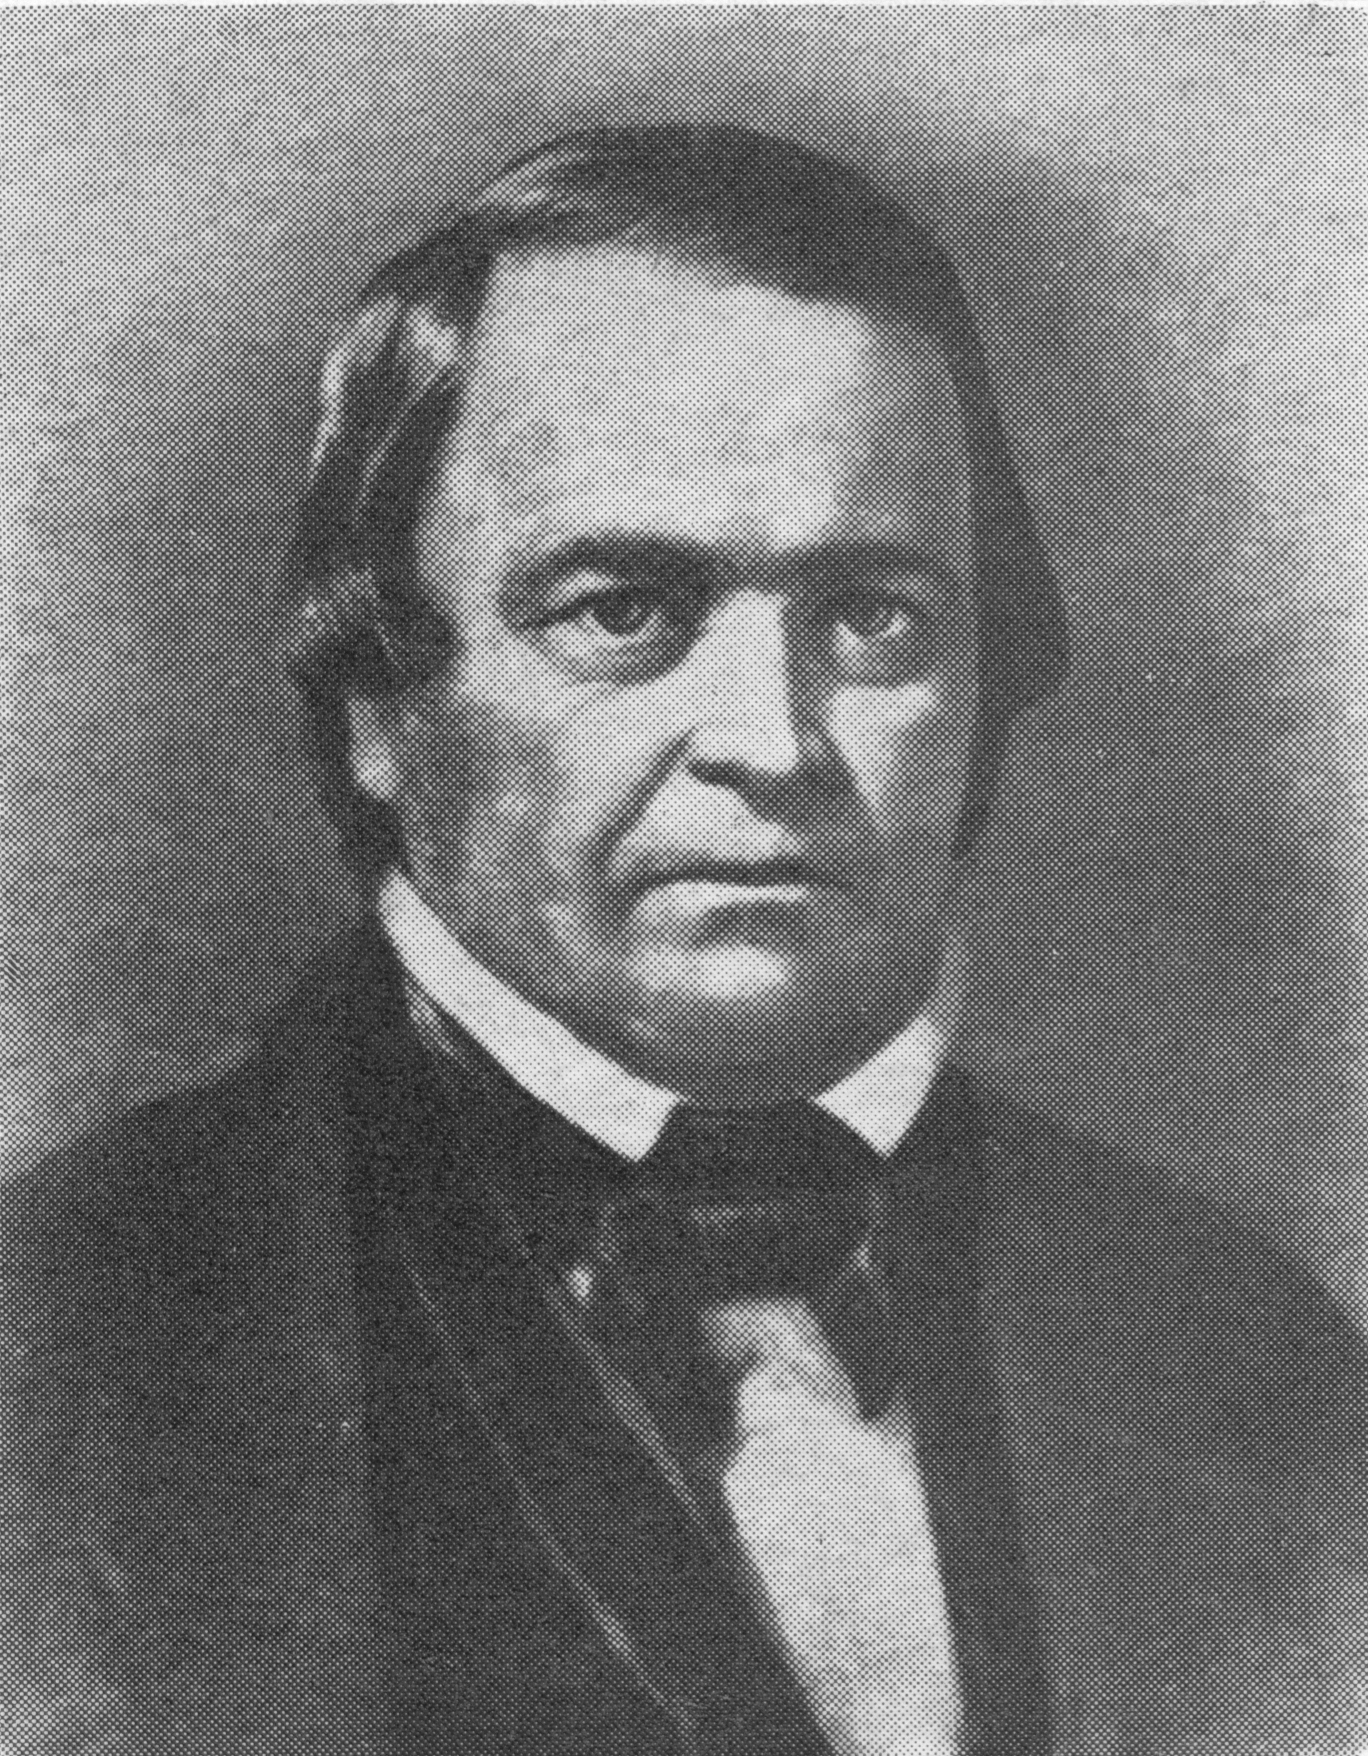
\includegraphics[width=1\linewidth]{images/william-miller.jpg}
    \caption*{William Miller (1782-1849)}
    \label{fig:w-miller}
\end{figure}


\begin{figure}[hp]
    \centering
    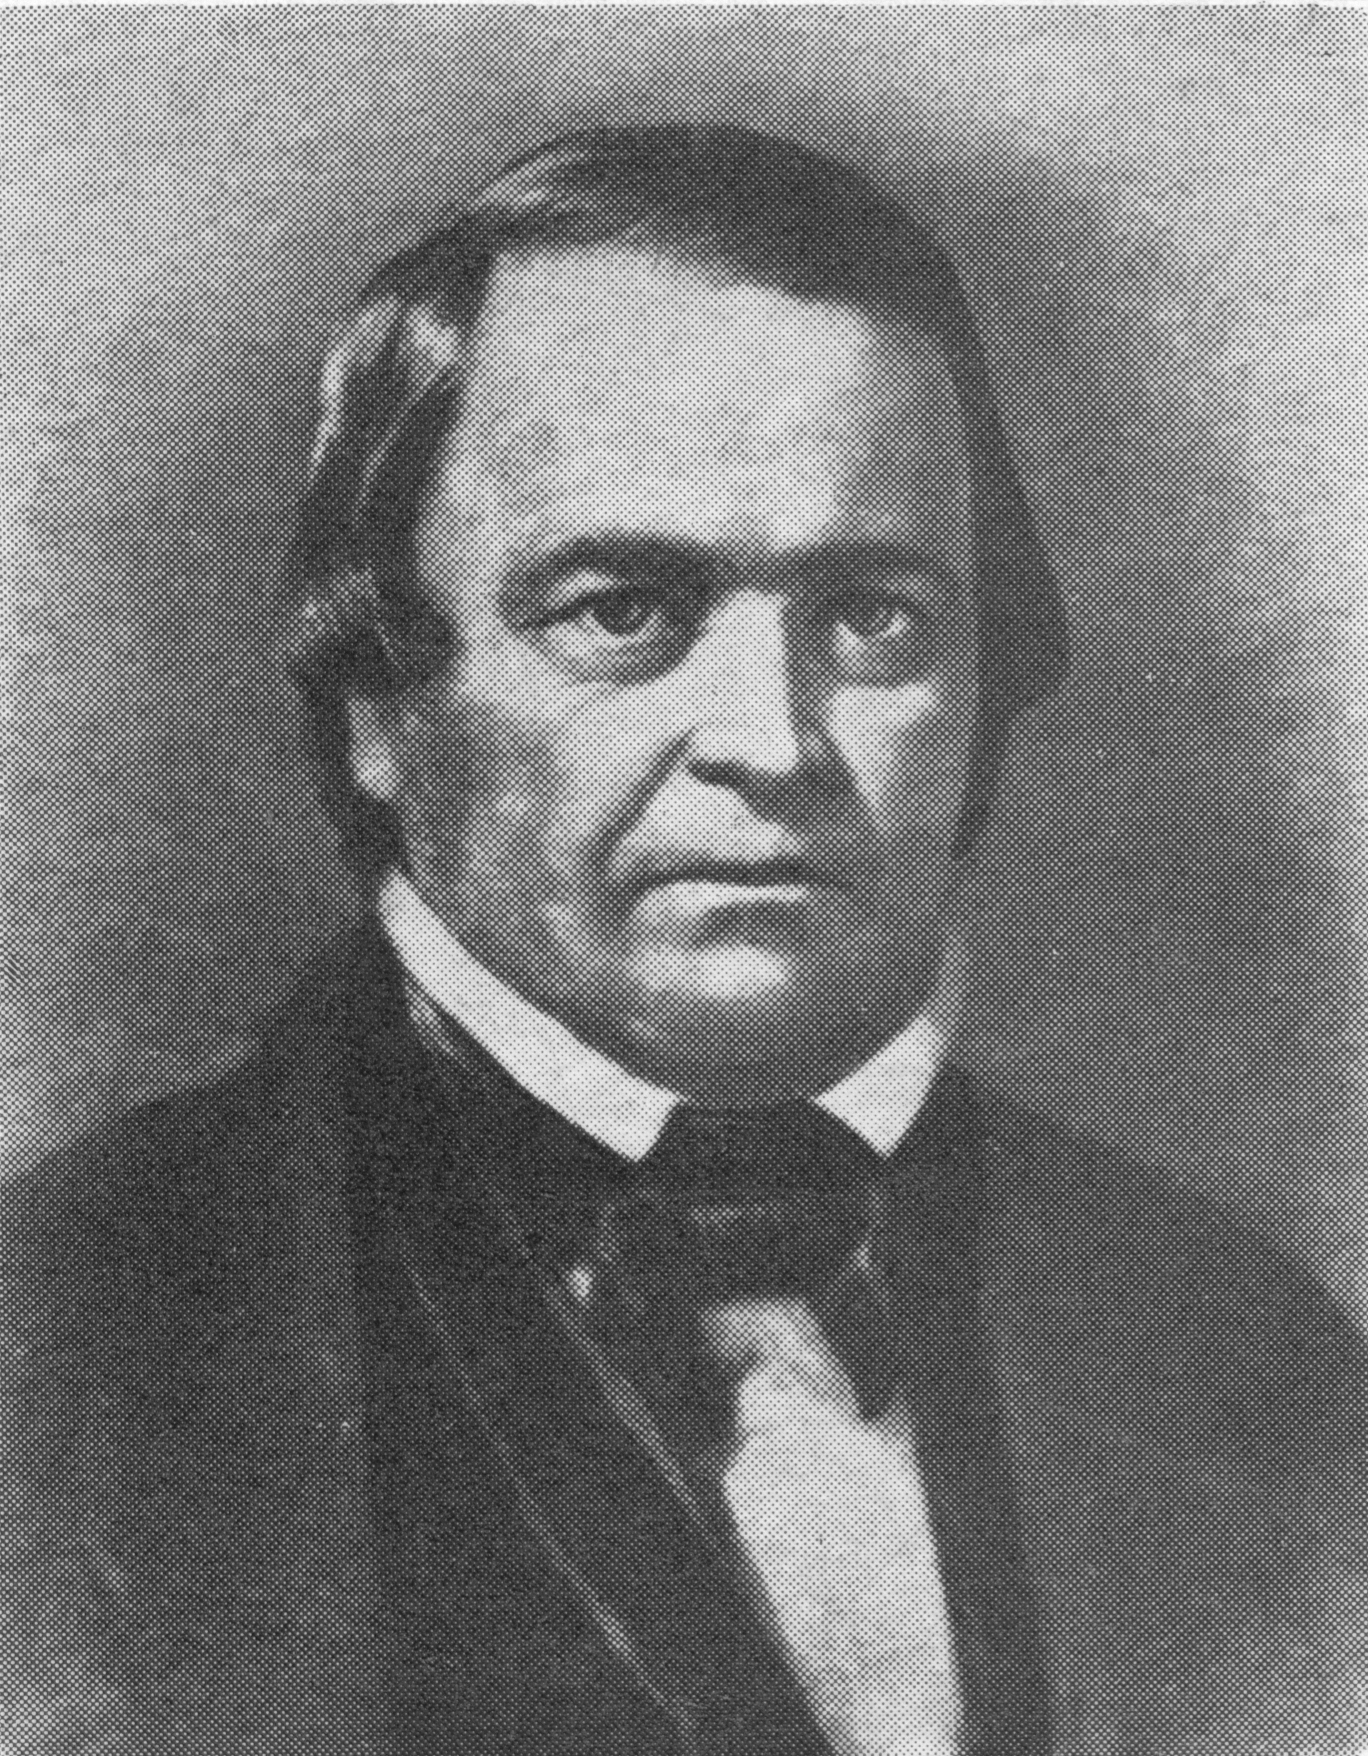
\includegraphics[width=1\linewidth]{images/william-miller.jpg}
    \caption*{William Miller (1782-1849)}
    \label{fig:w-miller}
\end{figure}


In reading the explanation of the great disappointment, did you see the answer to the question, “\textit{who is God whose judgment has come}?” The first angel’s message from Revelation 14:7 aligns exactly with the prophetic time declared in Daniel 8:14. The judgment that has come was the investigative judgment, which started in 1844. The Bible clearly describes whose hour of judgment has come in the first angel’s message. Let us read it in the Bible and see Ellen White’s comment.


Al leer la explicación del gran chasco, ¿vieron la respuesta a la pregunta, “\textit{quién es el Dios cuyo juicio ha venido}?” El mensaje del primer ángel de Apocalipsis 14:7 se alinea exactamente con el tiempo profético declarado en Daniel 8:14. El juicio que ha llegado era el juicio investigador, que comenzó en 1844. La Biblia describe claramente cuya hora de juicio ha llegado en el mensaje del primer ángel. Leámoslo en la Biblia y veamos el comentario de Ellen White.


\egw{‘I beheld,’ says the prophet Daniel, \textbf{‘till thrones were placed, and One that was \underline{Ancient of Days} \underline{did sit}}: \textbf{His raiment} was white as snow, and \textbf{the hair of His head} like pure wool; \textbf{His throne was fiery flames}, and the wheels thereof burning fire. A fiery stream issued and came forth from before Him: thousand thousands ministered unto Him, and ten thousand times ten thousand stood before Him: \textbf{\underline{the judgment was set, and the books were opened}}.’ Daniel 7:9, 10, R.V.}[GC 479.1; 1888][https://egwwritings.org/read?panels=p132.2169]


\egw{‘Contemplé -dice el profeta Daniel-, \textbf{‘hasta que se colocaron tronos, y se sentó uno que era el \underline{Anciano de Días}}: \textbf{su vestido} era blanco como la nieve, y \textbf{el cabello de su cabeza} como lana pura; \textbf{su trono era llamas de fuego}, y sus ruedas, fuego ardiente. Un torrente de fuego salía de delante de él; miles de miles le servían, y diez mil veces diez mil estaban de pie delante de él; \textbf{\underline{el juicio fue establecido, y los libros fueron abiertos}}.’ Daniel 7:9, 10, R.V.}[GC 479.1; 1888][https://egwwritings.org/read?panels=p132.2169]


\egwnogap{\textbf{Thus was presented to the prophet’s vision the great and solemn day when the characters and the lives of men should pass in review before the Judge of all the earth, and to every man should be rendered ‘according to his works.’ \underline{The Ancient of Days is God the Father}.} Says the psalmist: \textbf{‘Before }the mountains were brought forth, or ever Thou hadst formed the earth and the world, even \textbf{from everlasting to everlasting}, \textbf{Thou art God}.’ Psalm 90:2. \textbf{\underline{It is He, the source of all being, and the fountain of all law, that is to preside in the judgment}}. And holy angels as ministers and witnesses, in number ‘ten thousand times ten thousand, and thousands of thousands,’ attend this great tribunal.}[GC 479.2; 1888][https://egwwritings.org/read?panels=p132.2170]


\egwnogap{\textbf{Así se presentó a la visión del profeta el gran y solemne día en que los caracteres y las vidas de los hombres pasarían en revista ante el Juez de toda la tierra, y a cada hombre se le daría ‘según sus obras’. \underline{El Anciano de Días es Dios el Padre}.} Dice el salmista: \textbf{‘Antes de} que nacieran los montes, o de que formaras la tierra y el mundo, desde \textbf{la eternidad hasta la eternidad}, \textbf{tú eres Dios}.’ Salmo 90:2. \textbf{\underline{Es Él, la fuente de todo ser, y la fuente de toda ley, quien va a presidir el juicio}}. Y los santos ángeles como ministros y testigos, en número de ‘diez mil veces diez mil, y miles de miles,’ asisten a este gran tribunal.}[GC 479.2; 1888][https://egwwritings.org/read?panels=p132.2170]


\egwnogap{\textbf{‘And, behold, one like \underline{the Son of man} came with the clouds of heaven, and came to \underline{the Ancient of Days}, and they \underline{brought Him near before Him}}. And there was given Him dominion, and glory, and a kingdom, that all people, nations, and languages, should serve Him: His dominion is an everlasting dominion, which shall not pass away.’ Daniel 7:13, 14. \textbf{The coming of Christ here described is not His second coming to the earth}. \textbf{\underline{He comes to the Ancient of Days in heaven} to receive dominion and glory and a kingdom}, \textbf{which will be given Him at the close of His work as a mediator}. \textbf{\underline{It is this coming, and not His second advent to the earth, that was foretold in prophecy to take place at the termination of the 2300 days in 1844}}. \textbf{Attended by heavenly angels, our great High Priest enters the holy of holies and there appears in \underline{the presence of God}} to engage in the last acts of His ministration in behalf of man—\textbf{to perform the work of investigative judgment} and to \textbf{make an atonement} for all who are shown to be entitled to its benefits.}[GC 479.3; 1888][https://egwwritings.org/read?panels=p132.2171]


\egwnogap{\textbf{‘Y he aquí, uno como \underline{el Hijo del Hombre} vino con las nubes del cielo, y vino al \underline{Anciano de Días}, y lo \underline{acercaron delante de Él}}. Y le fue dado dominio, gloria y reino, para que todos los pueblos, naciones y lenguas le sirvieran: Su dominio es un dominio eterno, que no pasará’. Daniel 7:13, 14. \textbf{La venida de Cristo aquí descrita no es su segunda venida a la tierra}. \textbf{\underline{Viene al Anciano de Días en el cielo} para recibir dominio, gloria y reino}, \textbf{que le serán dados al final de su obra como mediador}. \textbf{\underline{Es esta venida, y no su segundo advenimiento a la tierra, lo que se predijo en la profecía que tendría lugar a la terminación de los 2300 días en 1844}}. \textbf{Asistido por los ángeles celestiales, nuestro gran Sumo Sacerdote entra en el lugar santísimo y allí aparece en \underline{presencia de Dios}} para realizar los últimos actos de su ministerio en favor del hombre—\textbf{llevar a cabo la obra del juicio investigador} y \textbf{hacer una expiación} por todos los que han demostrado tener derecho a sus beneficios.}[GC 479.3; 1888][https://egwwritings.org/read?panels=p132.2171]


The answer is simple and straightforward: The God of our pioneers was the Ancient of Days. \egwinline{The Ancient of Days is God the Father}. He is \textit{a personal}, \textit{spiritual being}. We see this in His description: \bible{Whose garment was white as snow, and the hair of his head like the pure wool: his throne was like the fiery flame, and his wheels as burning fire.}[Daniel 7:9]. In the termination of the 2300 days prophecy, in 1844, \bible{The hour of His judgment has come}[Revelation 14:7], \bible{the Ancient of days did sit} and \bible{the judgment was set, and the books were opened.}[Daniel 7:9,10]. The God from the first angel’s message is the Ancient of Days. Our pioneers were not ignorant regarding the truth about God. They believed \others{That there is \textbf{one God}, \textbf{\underline{a personal, spiritual being}}, \textbf{the creator of all things}, omnipotent, omniscient, and eternal, infinite in wisdom, holiness, justice, goodness, truth, and mercy; unchangeable, and \textbf{\underline{everywhere present by his representative, the Holy Spirit}}. Ps. 139:7.}[First point of the Fundamental Principles.] This one God is the Father, the Ancient of Days, \others{the creator of all things}, and we are to \bible{worship Him that made heaven, and earth, and the sea, and the fountains of waters}[Revelation 14:7]. He \bible{created all things by Jesus Christ}[Ephesians 3:9].


La respuesta es simple y directa: El Dios de nuestros pioneros era el Anciano de Días. \egwinline{El Anciano de días es Dios el Padre}. Él es \textit{un ser personal}, \textit{espiritual}. Lo vemos en su descripción: \bible{Cuyo vestido era blanco como la nieve, y el pelo de su cabeza como la lana pura; su trono era como llama de fuego, y sus ruedas como fuego ardiente.}[Daniel 7:9]. En la terminación de la profecía de los 2300 días, en 1844, \bible{La hora de su juicio ha llegado}[Apocalipsis 14:7], \bible{el Anciano de días se sentó} y \bible{el juicio fue establecido, y los libros fueron abiertos.}[Daniel 7:9,10]. El Dios del mensaje del primer ángel es el Anciano de Días. Nuestros pioneros no eran ignorantes respecto a la verdad sobre Dios. Creían \others{Que hay \textbf{un solo Dios}, \textbf{\underline{un ser personal y espiritual}}, \textbf{el creador de todas las cosas}, omnipotente, omnisciente y eterno, infinito en sabiduría, santidad, justicia, bondad, verdad y misericordia; inmutable y \textbf{\underline{presente en todas partes por medio de su representante, el Espíritu Santo}}. Sal. 139:7.}[Primer punto de los Principios Fundamentales.] Este único Dios es el Padre, el Anciano de Días, \others{el creador de todas las cosas}, y debemos \bible{adorar al que hizo el cielo, la tierra, el mar y las fuentes de las aguas}[Apocalipsis 14:7]. Él \bible{creó todas las cosas por medio de Jesucristo}[Efesios 3:9].


Today, the first angel’s message has not lost any of its importance. The messages of the second and third angel’s depend on the first message and only the first message requires action on our part. We are to worship God. More specifically, we are to worship the right God. In the last and final conflict, there will be two kinds of worshippers, as we have been told in Revelation 13 and 14.


Hoy, el mensaje del primer ángel no ha perdido nada de su importancia. Los mensajes del segundo y tercer ángel dependen del primer mensaje y sólo el primer mensaje requiere acción de nuestra parte. Debemos adorar a Dios. Más específicamente, debemos adorar al Dios correcto. En el último y definitivo conflicto, habrá dos clases de adoradores, como se nos ha dicho en Apocalipsis 13 y 14.


\bible{And all that dwell upon the earth shall \textbf{worship him} \normaltext{[the beast]}, \textbf{whose names are not written in the book of life of the Lamb} slain from the foundation of the world.}[Revelation 13:8]


\bible{Y todos los que habitan en la tierra \textbf{le adorarán} \normaltext{[a la bestia]}, \textbf{cuyos nombres no están escritos en el libro de la vida del Cordero} inmolado desde la fundación del mundo.}[Apocalipsis 13:8]


The group that worships the beast will receive the mark of the beast. The whole world will be compelled to worship the beast and his image with the threat of death.


El grupo que adore a la bestia recibirá la marca de la bestia. El mundo entero será obligado a adorar a la bestia y a su imagen con la amenaza de muerte.


\bible{And he \normaltext{[the beast]} had power to give life unto \textbf{the image of the beast}, that the image of the beast should both speak, and cause that \textbf{as many as would not worship the image of the beast should be killed}.}[Revelation 13:15]


\bible{Y él \normaltext{[la bestia]} tenía poder para dar vida a \textbf{la imagen de la bestia}, para que la imagen de la bestia hablara y para hacer que \textbf{todos los que no adorasen la imagen de la bestia fuesen muertos}.}[Apocalipsis 13:15]


We should not participate in this worship. Let us learn and have faith just like Daniel’s three friends who refused to worship the image of King Nebuchadnezzar. The beast represented in Revelation 13, that extorts the consciences of men by the peril of their lives, is the papacy. Dear friend, don't be fooled. The papal God is a Trinity God. Do not overlook that.


No debemos participar en esta adoración. Aprendamos y tengamos fe como los tres amigos de Daniel que se negaron a adorar la imagen del rey Nabucodonosor. La bestia representada en Apocalipsis 13, que extorsiona las conciencias de los hombres con el peligro de sus vidas, es el papado. Querido amigo, no te dejes engañar. El Dios papal es un Dios de la trinidad. No pases eso por alto.


We should worship the Ancient of Days as it is proclaimed in the first angel’s message. This is God the Creator who created everything through His Son, Jesus Christ. This is God from the first point of the \emcap{Fundamental Principles}. Our pioneers got this right.


Debemos adorar al Anciano de los Días como se proclama en el mensaje del primer ángel. Este es el Dios Creador que creó todo a través de su Hijo, Jesucristo. Este es Dios desde el primer punto de los \emcap{Principios Fundamentales}. Nuestros pioneros lo entendieron bien.


True understanding of the mission and purpose of the Seventh-day Adventist movement should be conclusive evidence that the Trinity doctrine is a foreign doctrine to us. We’ve ended up where we are today because we have forgotten \egwinline{\textbf{the way the Lord has led us, and \underline{His teaching} in our past history.}}[LS 196.2; 1915][https://egwwritings.org/read?panels=p41.1083] It is very sad to see how our Adventist scholars claim that our pioneers did not correctly understand the doctrine of God. If that were true, our pioneers would have failed to proclaim the first angel's message. They did not fail. We have failed.


La verdadera comprensión de la misión y el propósito del movimiento adventista del séptimo día debería ser una prueba concluyente de que la doctrina trinitaria es una doctrina extraña para nosotros. Hemos terminado donde estamos hoy porque hemos olvidado \egwinline{\textbf{la manera como el Señor nos ha guiado, y \underline{su enseñanza} en nuestra historia pasada.}}[LS 196.2; 1915][https://egwwritings.org/read?panels=p41.1083] Es muy triste ver cómo nuestros eruditos adventistas afirman que nuestros pioneros no entendieron correctamente la doctrina de Dios. Si eso fuera cierto, nuestros pioneros habrían fallado al proclamar el mensaje del primer ángel. Ellos no fallaron. Nosotros hemos fallado.


\others{\textbf{Most of the founders of Seventh-day Adventism would not be able to join the church today if they had to subscribe to the denomination's Fundamental Beliefs}.}\others{\textbf{More specifically, most would not be able to agree to belief number 2, which deals with the doctrine of the Trinity.} For Joseph Bates the Trinity was an unscriptural doctrine, for James White it was that “old Trinitarian absurdity,” and for M. E. Cornell it was a fruit of the great apostasy, along with such false doctrines as Sunday-keeping and the immortality of the soul.}[George Night, Ministry Magazine, October 1993][https://www.ministrymagazine.org/archive/1993/10/adventists-and-change]


\others{\textbf{La mayoría de los fundadores del Adventismo del Séptimo Día no podrían unirse a la iglesia hoy si tuvieran que suscribir las creencias fundamentales de la denominación}.}\others{\textbf{Más concretamente, la mayoría no podría estar de acuerdo con la creencia número 2, que trata de la doctrina de la trinidad.} Para Joseph Bates la trinidad era una doctrina no bíblica, para James White era ese ‘viejo absurdo trinitario’, y para M. E. Cornell era un fruto de la gran apostasía, junto con doctrinas falsas como la observancia del domingo y la inmortalidad del alma.}[George Night, Ministry Magazine, October 1993][https://www.ministrymagazine.org/archive/1993/10/adventists-and-change]


The doctrine of Trinity is the doctrine that undermines the foundation of our faith, the foundation that was laid at the beginning of our work. The distinction between truth and error lies in hermeneutics—the method of interpreting the Bible. Let us thoroughly investigate this issue.


La doctrina de la trinidad es la doctrina que socava los cimientos de nuestra fe, los cimientos que se pusieron al principio de nuestra obra. La distinción entre la verdad y el error radica en la hermenéutica—el método de interpretar la Biblia. Investiguemos a fondo este asunto.


\begin{titledpoem}
\stanza{
    In faith's first light, they sought His face, \\
    A vision pure, of divine grace. \\
    The pioneers, with vision clear, \\
    In 1844, held God so dear.
}

\stanza{    
    "The hour of judgment has come," they cried, \\
    To a world, both far and wide. \\
    The Ancient of Days, they did proclaim, \\
    Not a trinity, but a singular name.
}

\stanza{    
    Ellen White, with pen in hand, \\
    Spoke of a sanctuary, not of earthly land. \\
    A message of heaven, pure and bright, \\
    Guiding the faithful through the night.
}

\stanza{    
    The first angel’s message, a call to revere, \\
    God the Father, whom we should fear. \\
    "Who is the God we are to adore?" \\
    Not a trinity—this, they implored.
}

\stanza{    
    The Trinity, a concept unembraced, \\
    By pioneers, who in God's word traced. \\
    The Father, the Ancient, they did declare, \\
    His judgment and mercy, beyond compare.
}

\stanza{
    Yet, whispers now, through time have spread, \\ 
    A trinity's shadow, causing dread. \\
    If this be the God they were to declare, \\
    Their mission failed, caught in despair.
}

\stanza{
    But this is a falsehood, bold and cold, \\
    A narrative modern, but wrongly told. \\
    The Father they worshiped, with fervent zeal, \\
    Was the true God, their mission real.
}

\stanza{
    In unity, may we seek His face, \\
    Embracing truth, with grace and grace. \\
    The pioneers' vision, let us not lose, \\
    For in their footsteps, we must choose.
}

\stanza{
    To worship the God, of days of old, \\
    The Ancient of Days, as was foretold. \\
    In Revelation’s message, clear and bright, \\
    Guiding us still, through darkest night.
}
\end{titledpoem}


\begin{titledpoem}
\stanza{
    In faith's first light, they sought His face, \\
    A vision pure, of divine grace. \\
    The pioneers, with vision clear, \\
    In 1844, held God so dear.
}

\stanza{    
    "The hour of judgment has come," they cried, \\
    To a world, both far and wide. \\
    The Ancient of Days, they did proclaim, \\
    Not a trinity, but a singular name.
}

\stanza{    
    Ellen White, with pen in hand, \\
    Spoke of a sanctuary, not of earthly land. \\
    A message of heaven, pure and bright, \\
    Guiding the faithful through the night.
}

\stanza{    
    The first angel’s message, a call to revere, \\
    God the Father, whom we should fear. \\
    "Who is the God we are to adore?" \\
    Not a trinity—this, they implored.
}

\stanza{    
    The Trinity, a concept unembraced, \\
    By pioneers, who in God's word traced. \\
    The Father, the Ancient, they did declare, \\
    His judgment and mercy, beyond compare.
}

\stanza{
    Yet, whispers now, through time have spread, \\ 
    A trinity's shadow, causing dread. \\
    If this be the God they were to declare, \\
    Their mission failed, caught in despair.
}

\stanza{
    But this is a falsehood, bold and cold, \\
    A narrative modern, but wrongly told. \\
    The Father they worshiped, with fervent zeal, \\
    Was the true God, their mission real.
}

\stanza{
    In unity, may we seek His face, \\
    Embracing truth, with grace and grace. \\
    The pioneers' vision, let us not lose, \\
    For in their footsteps, we must choose.
}

\stanza{
    To worship the God, of days of old, \\
    The Ancient of Days, as was foretold. \\
    In Revelation’s message, clear and bright, \\
    Guiding us still, through darkest night.
}
\end{titledpoem}
